% !TeX program = xelatex
% !TeX encoding = utf8
% !TeX root = Elo1_HS22.tex

%% TODO: publish to CTAN
\documentclass[margin=normal]{tex/hsrzf}

%%%%%%%%%%%%%%%%%%%%%%%%%%%%%%%%%%%%%%%%%%%%%%%%%%%
% Packages

%% TODO: publish to CTAN
\usepackage{tex/hsrstud}

%% Language configuration
\usepackage{polyglossia}
\usepackage{multicol}
\usepackage{tikz}
\usepackage[european]{circuitikz}
\usepackage{tabularx}
\usepackage{enumitem}
\usepackage{colortbl}
\usepackage{graphics}

%% Color Configutation


\setdefaultlanguage[variant=swiss]{german}

%% License configuration
\usepackage[
    type={CC},
    modifier={by-nc-sa},
    version={4.0},
    lang={german},
]{doclicense}

%%%%%%%%%%%%%%%%%%%%%%%%%%%%%%%%%%%%%%%%%%%%%%%%%%%
% Metadata

\course{Elektrotechnik}
\module{Elo1}
\semester{Herbstsemester 2022}

\authoremail{joel.leirer@ost.ch}
\author{\textsl{Joël Leirer} -- \texttt{\theauthoremail}}

% did someone help you with this work?
\contributors{

  % do not forget to add yourself!
}

\title{\texttt{\themodule} Zusammenfassung}
\date{\thesemester}

%%%%%%%%%%%%%%%%%%%%%%%%%%%%%%%%%%%%%%%%%%%%%%%%%%%
% Document

\begin{document}

% use roman numberals for introductiory pages
\pagenumbering{roman}

\maketitle

% \begin{abstract}
% \end{abstract}

% show the names of the people who contributed to this document.
% \section*{Contributors}
% \thecontributors

\section*{Lizenz}
\doclicenseThis

\subsection*{Note}
Erlaubte Unterlagen an Prüfung: 5x A4-Blätter Zusammenfassung \\
Weitere Hilfsmittel: Taschenrechner

\clearpage
\tableofcontents

% actual content
\clearpage
\setcounter{page}{1}
\pagenumbering{arabic}

\section{Arbeitspunktbestimmung}
AC und DC Teile der Schaltung separat anschauen.
\begin{multicols}{2}

  \subsection{DC}
  \begin{itemize}
    \item Grosssignalwiderstung ($\frac{U}{I}$)
    \item AC-Quellen "Abschalten", AC-Quellen mit DC Anteil durch DC-Quellen ersetzen
    \item Kondensatoren entfernen (Unterbruch)
    \item Spule Kurschliessen
  \end{itemize}
  \subsection{AC}
  \begin{itemize}
    \item Kleinsignalwiderstand (Impedanz,$\frac{dU}{dI}$)
    \item DC-Quellen "Abschalten"
    \item Nichtlineare Bauteile durch ihre Kleinsignal Ersatzschaltung ersetzen
    \item Kondensatoren $\to$ Widerstände $X_{jc}= \frac{1}{2\pi f C}$
    \item Sperrdrosseln ("grossse" Induktivitäten) entfernen (Unterbruch)
  \end{itemize}
\end{multicols}

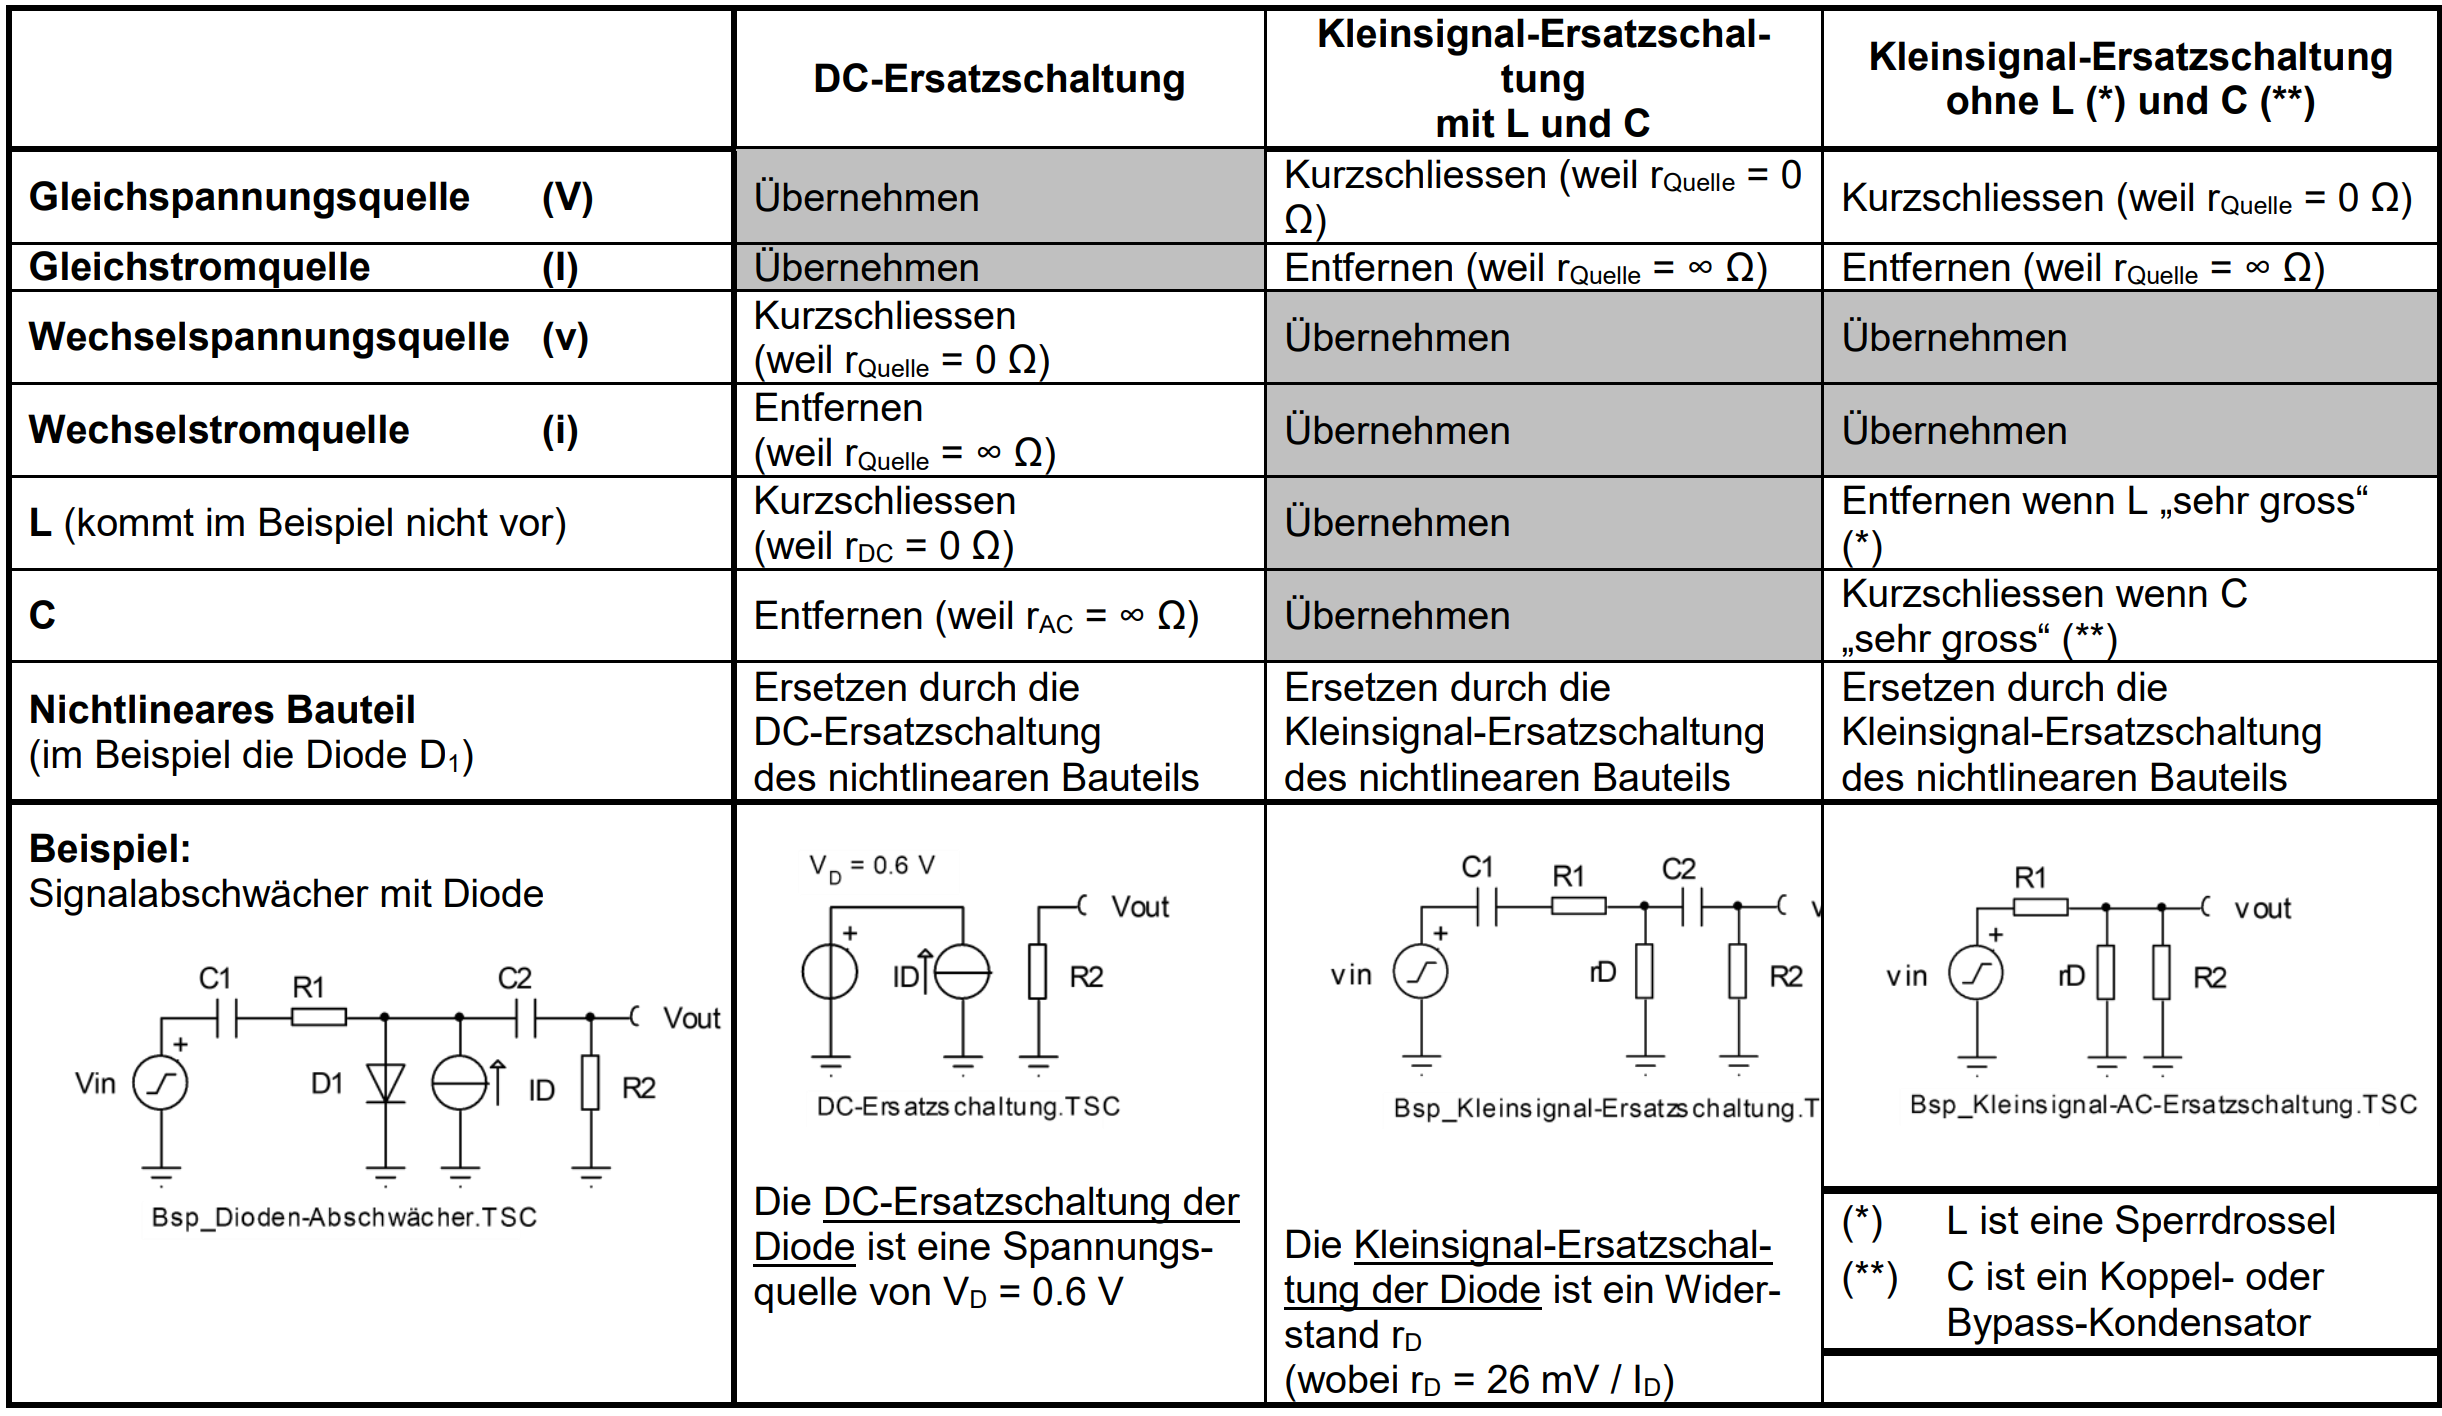
\includegraphics[width = 15cm]{img/Tabelle Kleinsignal Ersatzschaltung.png}
\newpage
\section{OpAmp}
\subsection{Schaltungen mit negativer Rückkopplung}
\begingroup
\small
\begin{tabularx}{0.8\textwidth}{p{155pt}p{155pt}p{155pt}}
  \textbf{Nicht Invertierender Verstärker}                                                          &
  \textbf{Invertierender Verstärker}                                                                &
  \textbf{Summierender Verstärker}                                                                    \\
  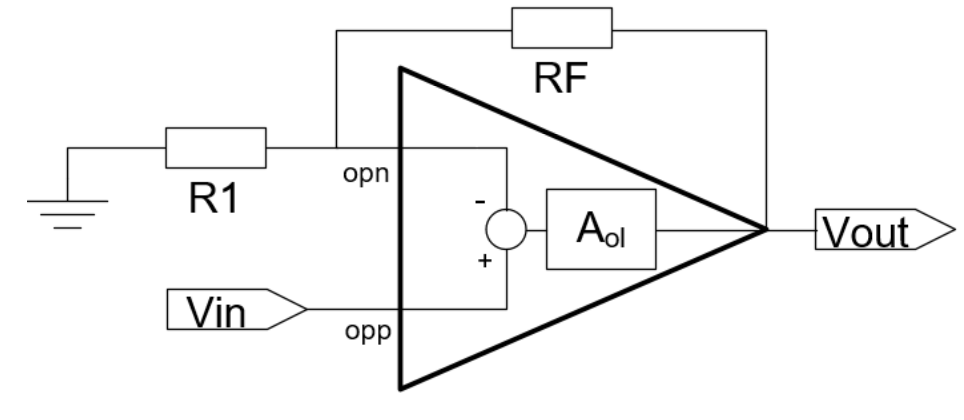
\includegraphics[width = 3.5cm]{img/OpAmp/Verstaerker_nicht_invertierend.png}                     &
  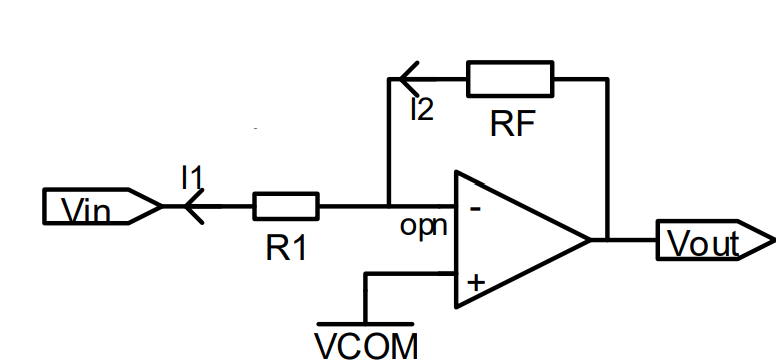
\includegraphics[width = 3.5cm]{img/OpAmp/Verstaerker_invertierend.png}                           &
  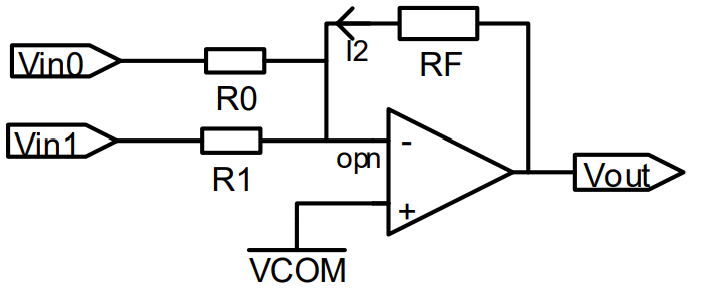
\includegraphics[width = 3.5cm]{img/OpAmp/Verstaerker_summierend.png}                               \\
  $ V_{out} = V_{in} \cdot (1 + \frac{R_F}{R_1})$                                                   &
  $ V_{out} = V_{RF} = -\frac{RF}{R_1}\cdot V_{in}$                                                 &
  $ V_{out} = RF \cdot I_2 = -RF \cdot (\frac{V_{in1}}{R_1} + \frac{V_{in0}}{R_0}) $                  \\
  \\
  \textbf{Buffer}                                                                                   &
  \textbf{Invertierender Addierer}                                                                  &
  \textbf{Gewichteter Subtrahierer}                                                                   \\
  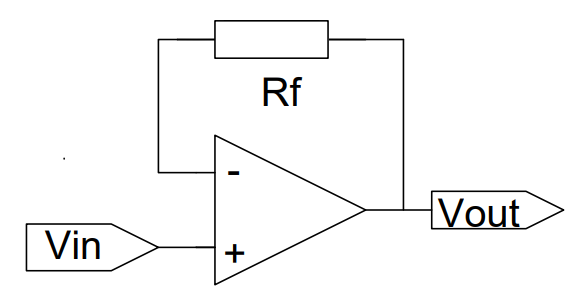
\includegraphics[width = 3.5cm]{img/OpAmp/Buffer.png}                                             &
  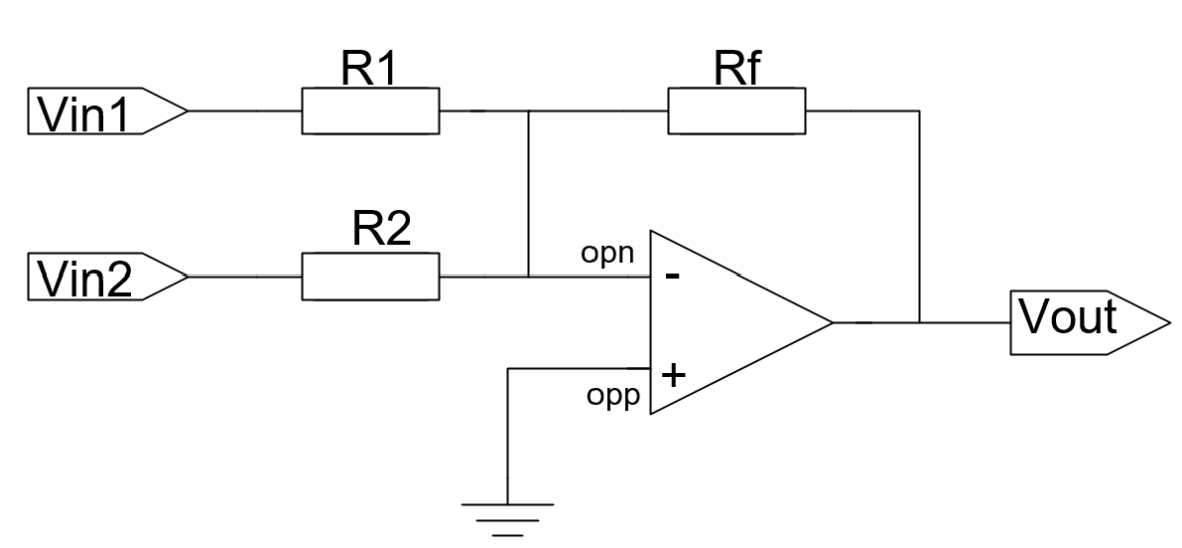
\includegraphics[width = 3.5cm]{img/OpAmp/Invertierender_Addierer.png}                            &
  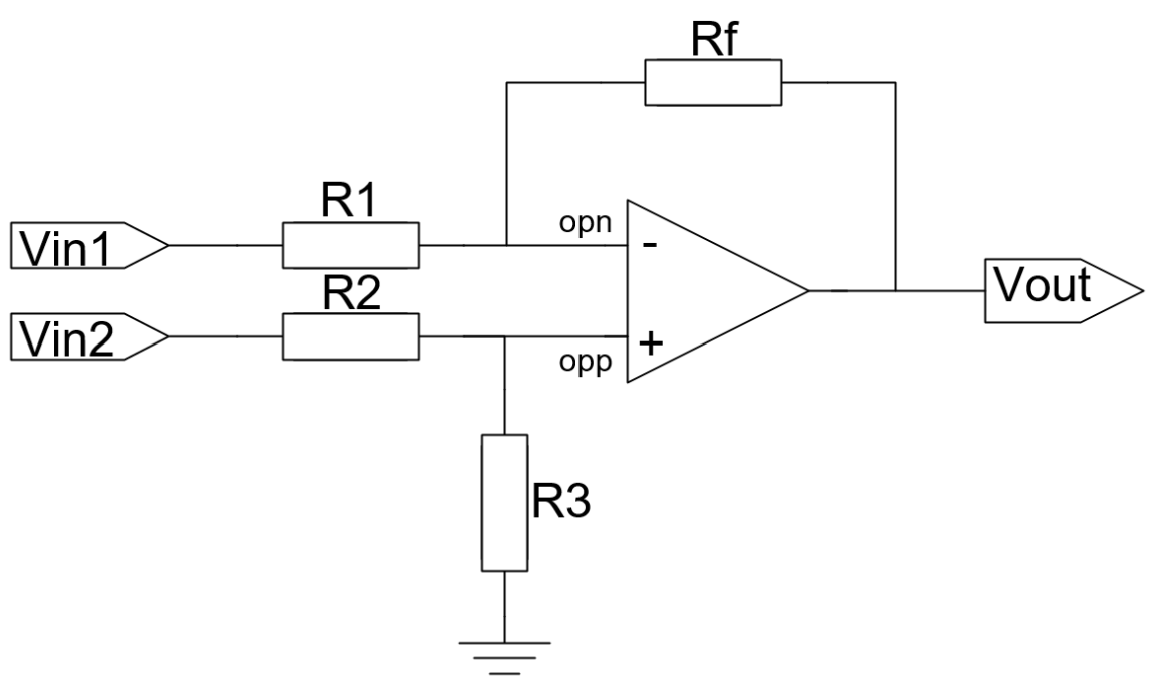
\includegraphics[width = 3.5cm]{img/OpAmp/Gewichteter_Subtrahierer.png}                             \\
  $ V_{out} = V_{in}$                                                                               &
  $ V_{out} = - RF \cdot (\frac{V_{in1}}{R_1} + \frac{V_{in2}}{R_2}) $                              &
  \resizebox{140pt}{!}
  {
    $ V_{out} =\frac{R_3}{R_3 + R_2} \cdot (1 + \frac{R_F}{R_1}) \cdot V_{in2} - \frac{R_F}{R_1} \cdot V_{in2}$
  }                                                                                                   \\
  \\
  \textbf{Differenzverstärker}                                                                      &
  \textbf{Instrumentenverstärker}                                                                   &
  \textbf{Mehrstufige Verstärker}                                                                     \\
  \includegraphics[width = 3.5cm]{img/OpAmp/Differenzverstärker.png}                                &
  \includegraphics[width = 3.5cm]{img/OpAmp/Instrumentenverstärker.png}                             &
  \includegraphics[width = 3.5cm]{img/OpAmp/Mehrstufige_Verstärker.png}                               \\
  \resizebox{140pt}{!}
  {
    $ V_{out} = \frac{R_3 + R_4}{R_3} \cdot (\frac{R_1}{R_1 + R_2} \cdot V_{AGND} + \frac{R_2}{R_1 + R_2} \cdot V_{in1}) - \cdot \frac{R_4}{R_3} \cdot V_{in2}$
  }
  \resizebox{100pt}{!}
  {
    \newline wenn $\frac{R_4}{R_3} = \frac{R_2}{R_1} \rightarrow V_{out} =\frac{R_4}{R_3} \cdot (V_{in1}-V_{in2})$
  }                                                                                                 &
  \resizebox{140pt}{!}
  {
    $ V_{out} = V_{ref} + \frac{R_4}{R_3} \cdot (1 + \frac{Rf1 + Rf2}{RG}) \cdot (V_{in2} - V_{in1})$
  }                                                                                                 &
  Verstärkung total $ A_{tot} = A_1 \cdot A_2 \cdot A_3\cdot\dots$                                    \\
  \\
  \textbf{Invertierender Verstärker \newline
  mit T-Glied in Rückkopplung}                                                                      &
  \textbf{Negativer Impedanz Konverter NIC}                                                           \\
  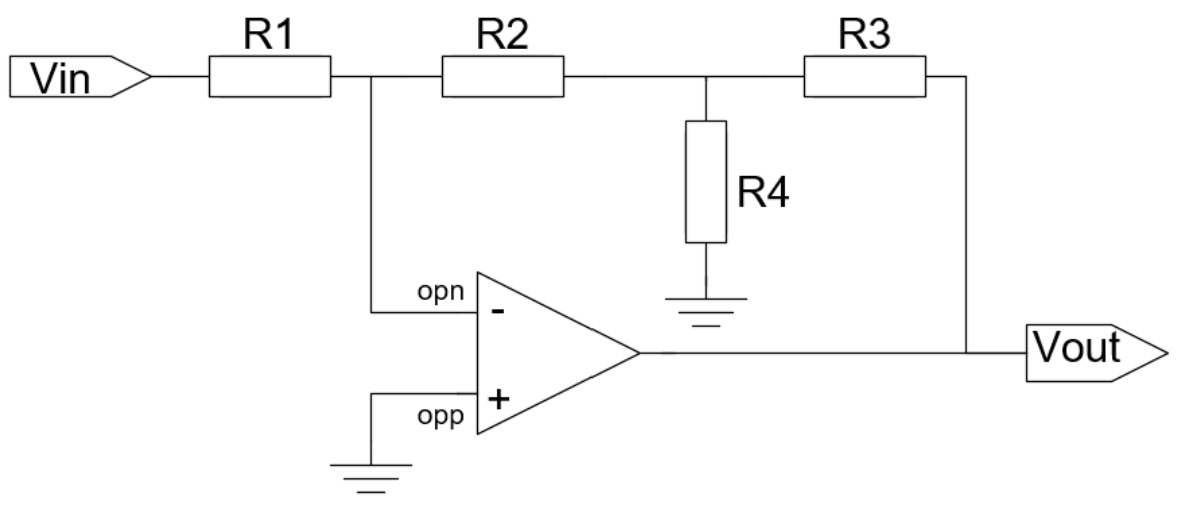
\includegraphics[width = 3.5cm]{img/OpAmp/Invertierender_Verstärker_mit_T-Glied_Rückkopplung.png} &
  \includegraphics[width = 3.5cm]{img/OpAmp/Negativer_Impedanz_Verstärker.png}                        \\
  $ V_{out} = - V_{in} \cdot \frac{R_2 + R_3 + \frac{R_2R_3}{R4}}{R_1} $
  \newline
  $ V_{out} = V_{in} \cdot (1+ \frac{R_2}{R_1})$                                                    &
  $R_{EQ} = -R \cdot \frac{R_1}{R_2}$
  \\
\end{tabularx}
\endgroup

\subsubsection{Gesteuerte Quellen}
\begingroup
\small
\begin{tabularx}{0.8\textwidth}{p{100pt}p{100pt}p{100pt}p{120pt}}
  \textbf{Spannungsgesteuerte \newline Stromquelle V1}                                         &
  \textbf{Spannungsgesteuerte \newline  Stromquelle V2}                                        &
  \textbf{Spannungsgesteuerte \newline Stromquelle \newline
  für geerdete Last RL}                                                                        &
  \textbf{Stromgesteuerte \newline Stromquelle}                                                  \\
  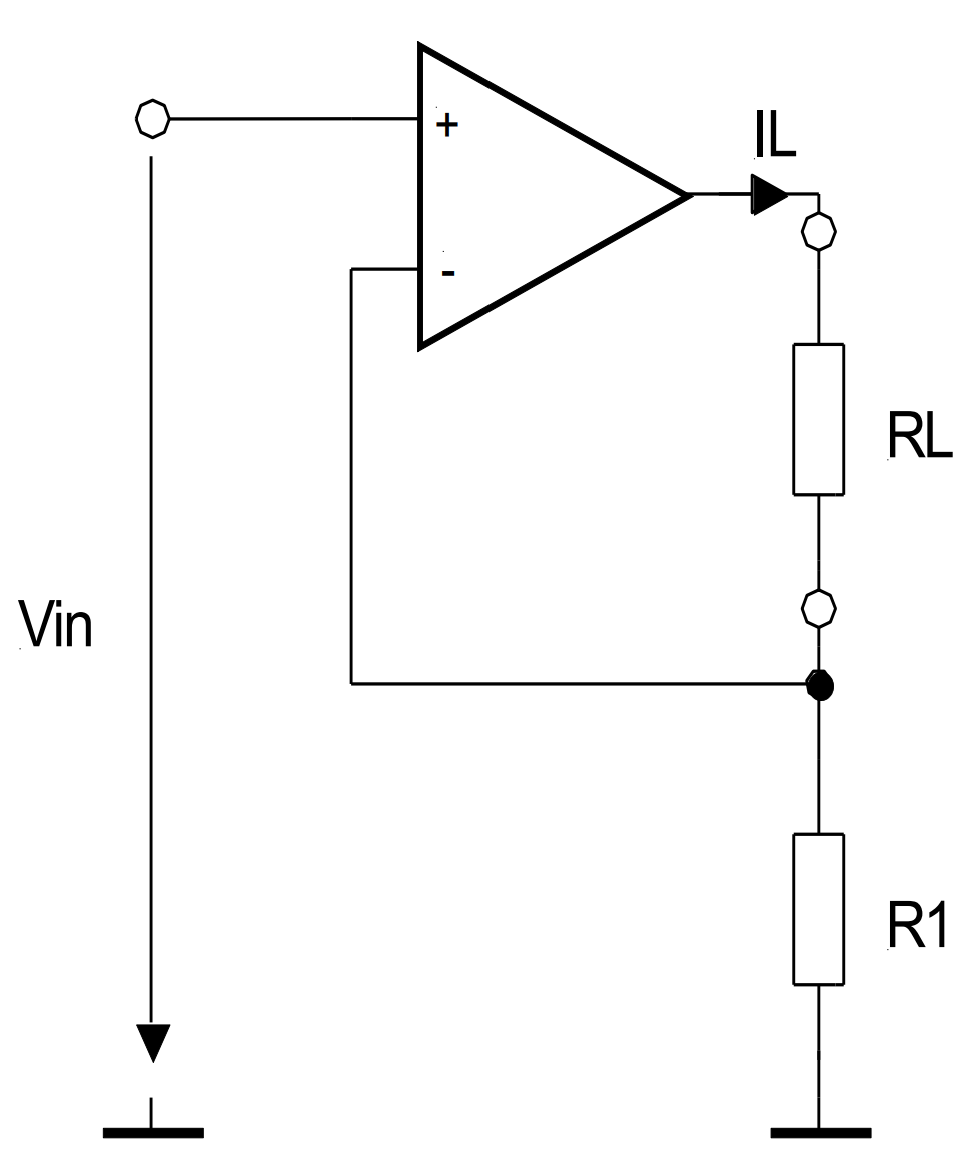
\includegraphics[width = 3.5cm]{img/OpAmp/Spannungsgesteuerte_Stromquelle_V1.png}            &
  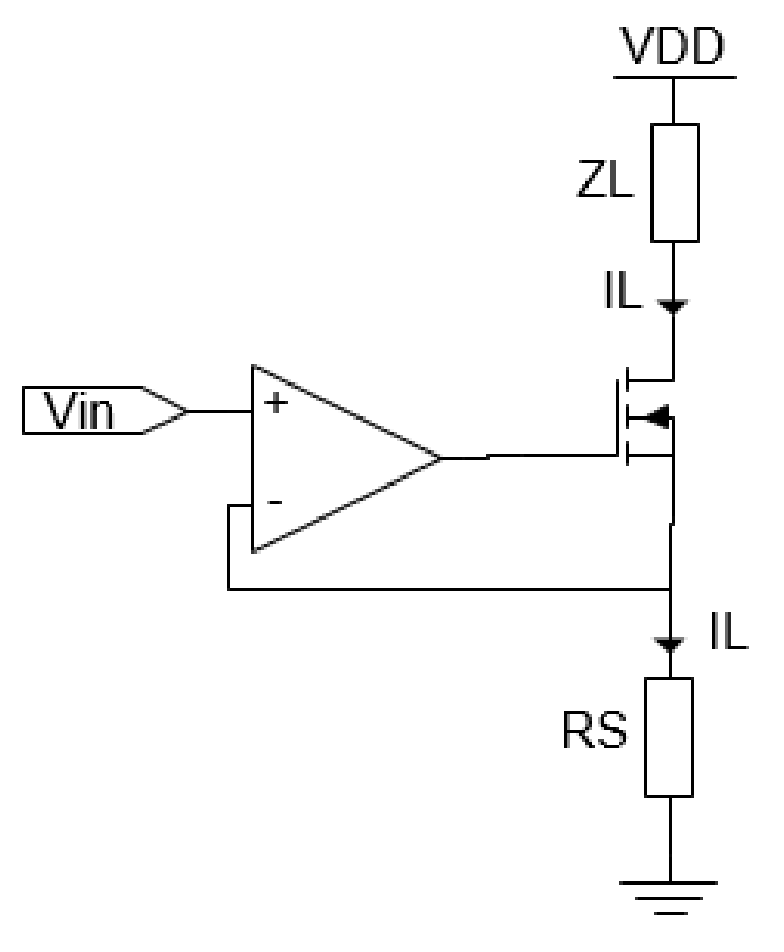
\includegraphics[width = 3.5cm]{img/OpAmp/Spannungsgesteuerte_Stromquelle_V2.png}            &
  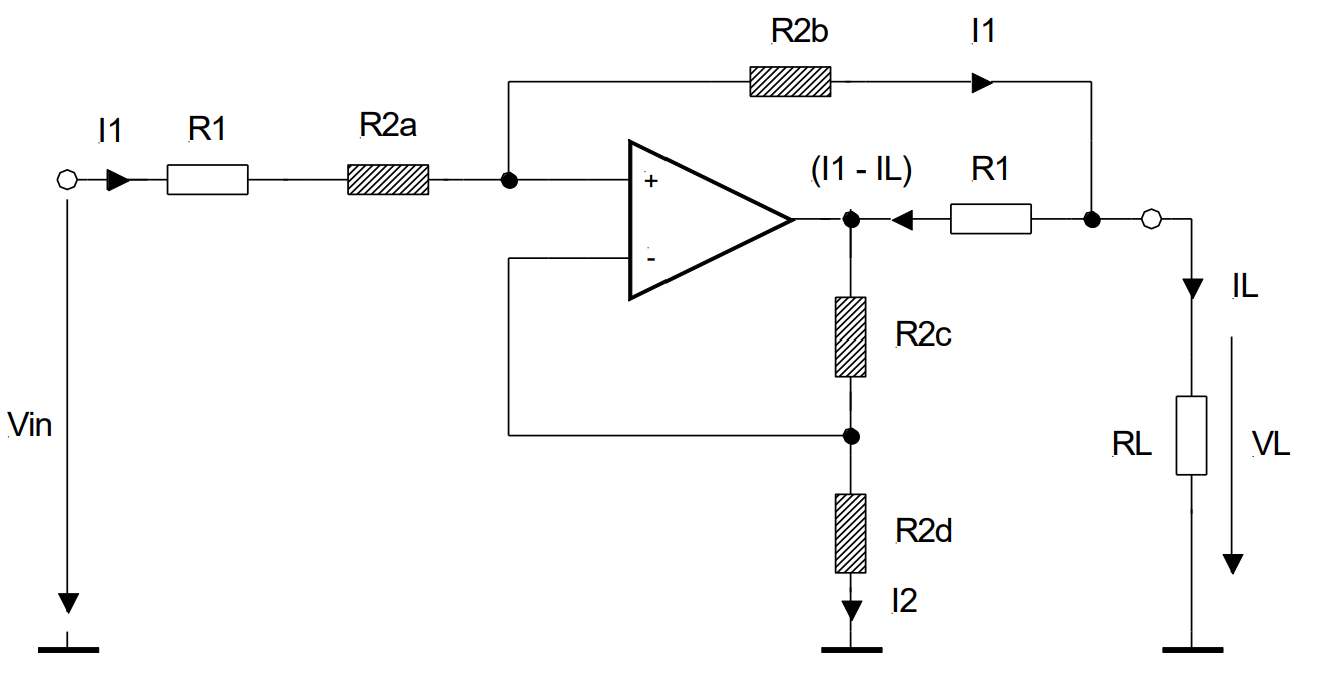
\includegraphics[width = 3.5cm]{img/OpAmp/Spannungsgesteuerte_Stromquelle_geerdete_Last.png} &
  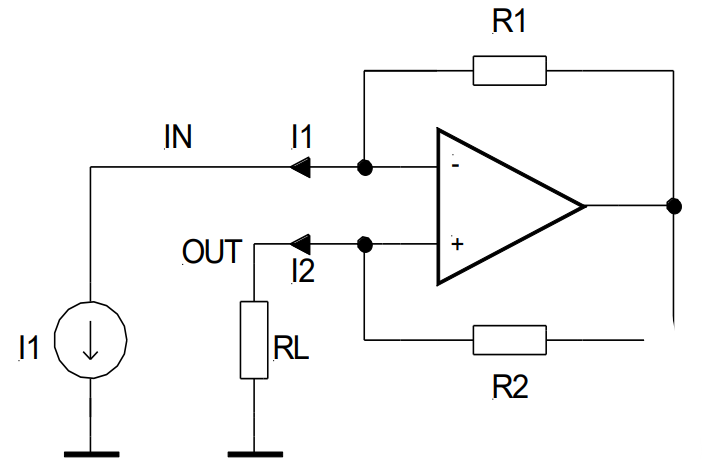
\includegraphics[width = 3.5cm]{img/OpAmp/Stromgesteuerte_Stromquelle.png}                     \\
  $ I_L = \frac{V_{in}}{R_1} $                                                                 &
  $ I_L = \frac{V_{in}}{R_S} $                                                                 &
  $ I_L = \frac{V_{in}}{R_1} $                                                                 &
  $ R_1I_1=R_2I_2; \; A_i = \frac{I_2}{I_1} = \frac{R_1}{R_2}  $
\end{tabularx}
\endgroup

\subsubsection{Filterschaltungen}
\begingroup
\small
\begin{tabularx}{\textwidth}{p{155pt}p{155pt}p{155pt}}
  \textbf{RC-Integrator}                                                                        &
  \textbf{Differenzierer}                                                                       &
  \textbf{Tiefpass-Filter}                                                                        \\
  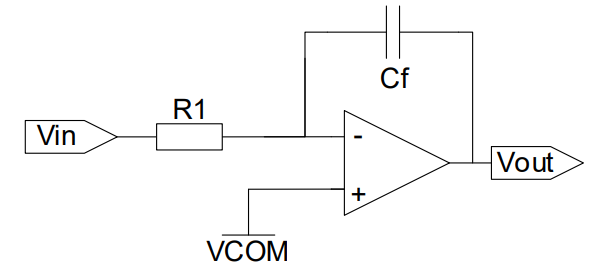
\includegraphics[width=3.5cm]{img/OpAmp/RC-Integrator.png}                                    &
  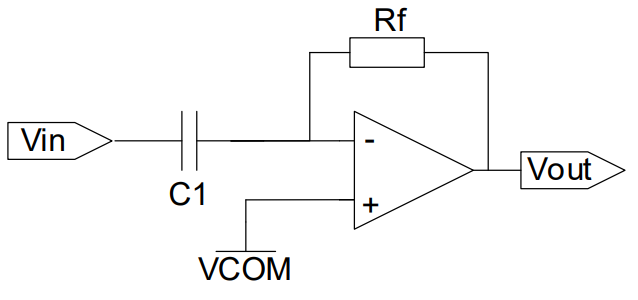
\includegraphics[width=3.5cm]{img/OpAmp/Differenzierer.png}                                   &
  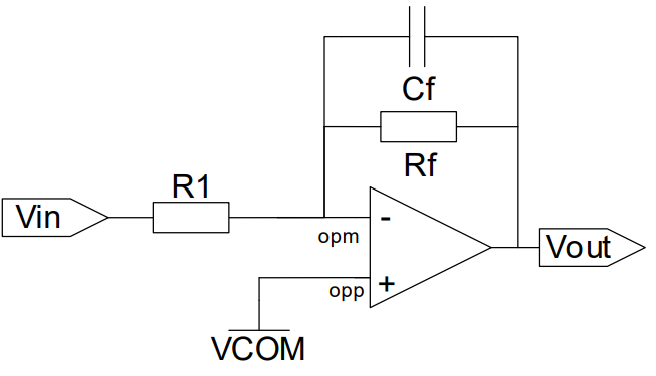
\includegraphics[width=3.5cm]{img/OpAmp/TiefpassFilter.png}                                     \\
  $V_{out}(t) = -\frac{1}{C} \int \limits _0 ^t i_c(\tau) d\tau + V_c(t=0)$
  \newline $V_{out}(t) = -\frac{1}{R \cdot C} \int \limits _0 ^t V_{in}(\tau) d\tau + V_c(t=0)$ &
  $V_{out} = -R_FC_1\frac{dv_{in}}{dt}$
  \newline  $i_c = C_1\frac{dv_c}{dt} = C_1\frac{dv_{in}}{dt} $                                 &
  Grenzfrequenz: $\frac{1}{2\pi R C} $
  \newline DC: $I_C = 0; \; V_{out} = -\frac{Rf}{R1}\cdot V_{in}$                                 \\
  \textbf{Bandpass-Filter}                                                                      &
  \textbf{Allpass-Filter}                                                                       &
  \\
  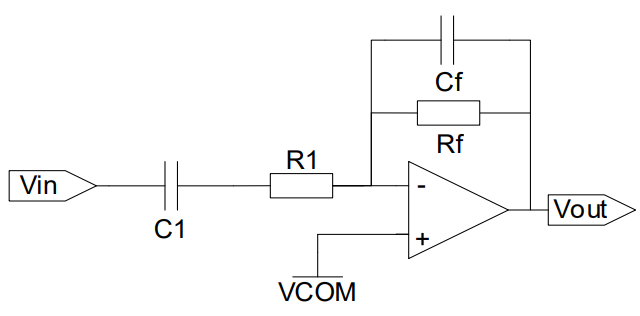
\includegraphics[width=3.5cm]{img/OpAmp/BandPass.png}                                         &
  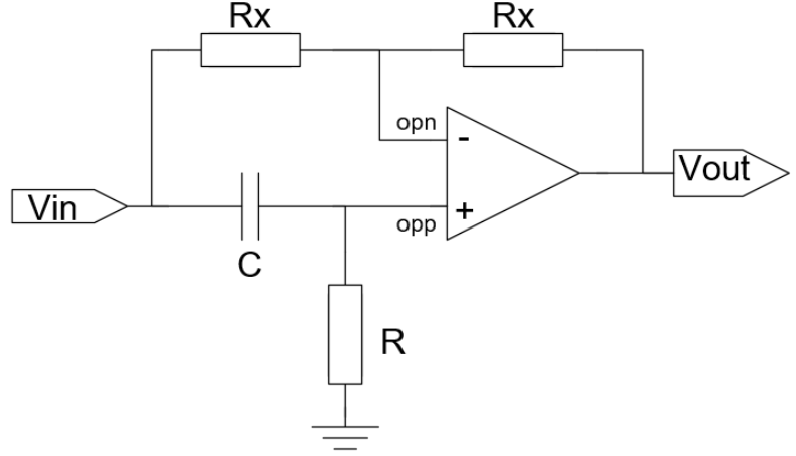
\includegraphics[width=3.5cm]{img/OpAmp/AllPass.png}                                          &
  \\
  $\omega_1 = \frac{1}{R_1\cdot C_1}$
  $\omega_2 = \frac{1}{R_F \cdot C_F}$
\end{tabularx}
\endgroup

\begin{multicols}{2}
  \subsection{OpAmp als Komparator}
  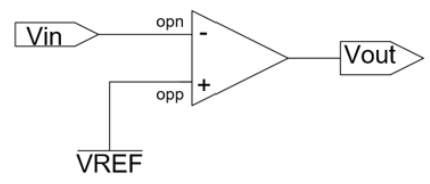
\includegraphics[width=3cm]{img/OpAmp/Komparator.png}\\
  $V_{out} = V_{mitte} = \frac{V_{pos} + V_{neg}}{2}$
  \subsubsection*{Schmitt-Trigger (nicht invertierend)}

  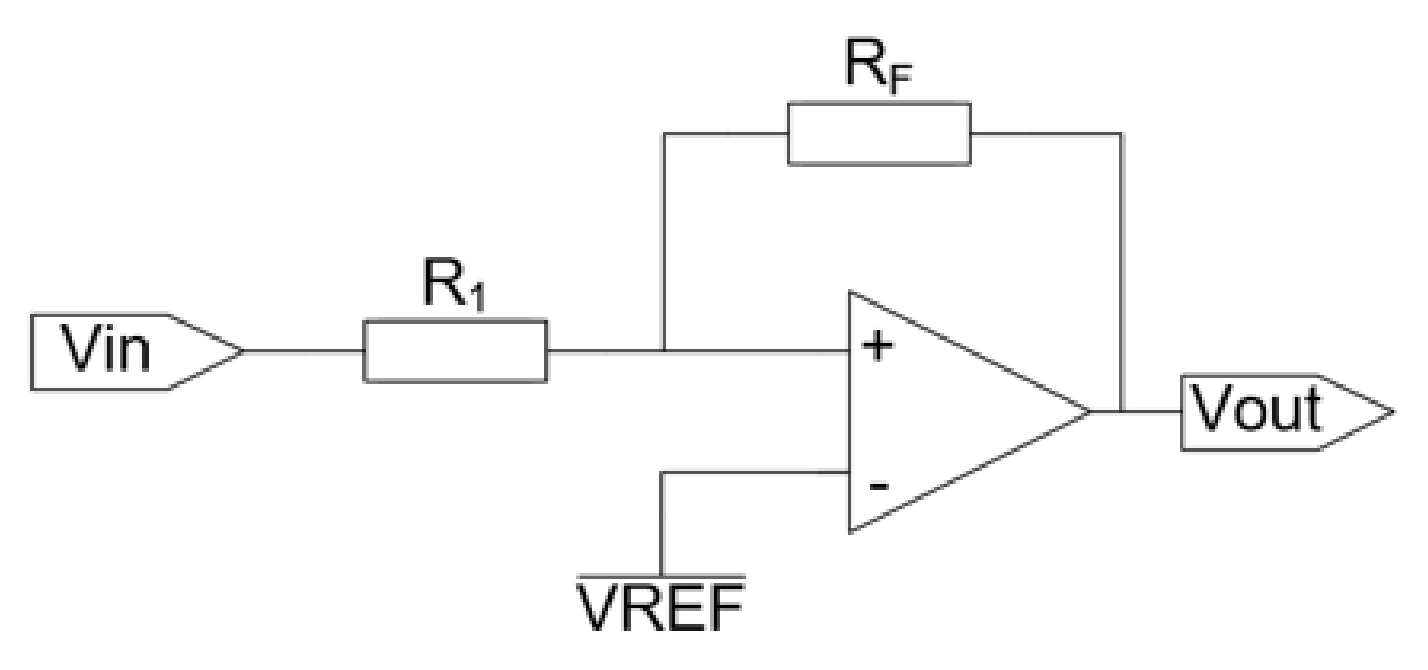
\includegraphics[width=3cm]{img/OpAmp/Schmitt-Trigger_nicht_invertierend.png}


  $V_{T_+} = V_{ref} + (V_{ref} - V_{out min})\frac{R_1}{R_F} $ \\
  $V_{T_-} = V_{ref} + (V_{out max} - V_{ref})\frac{R_1}{R_F} $\\
  $V_H = V_{T_+} - V_{T_-} = (V_{outmax} - V_{outmin})\frac{R_1}{R_F}$

  \subsubsection*{Schmitt Trigger (invertierend)}
  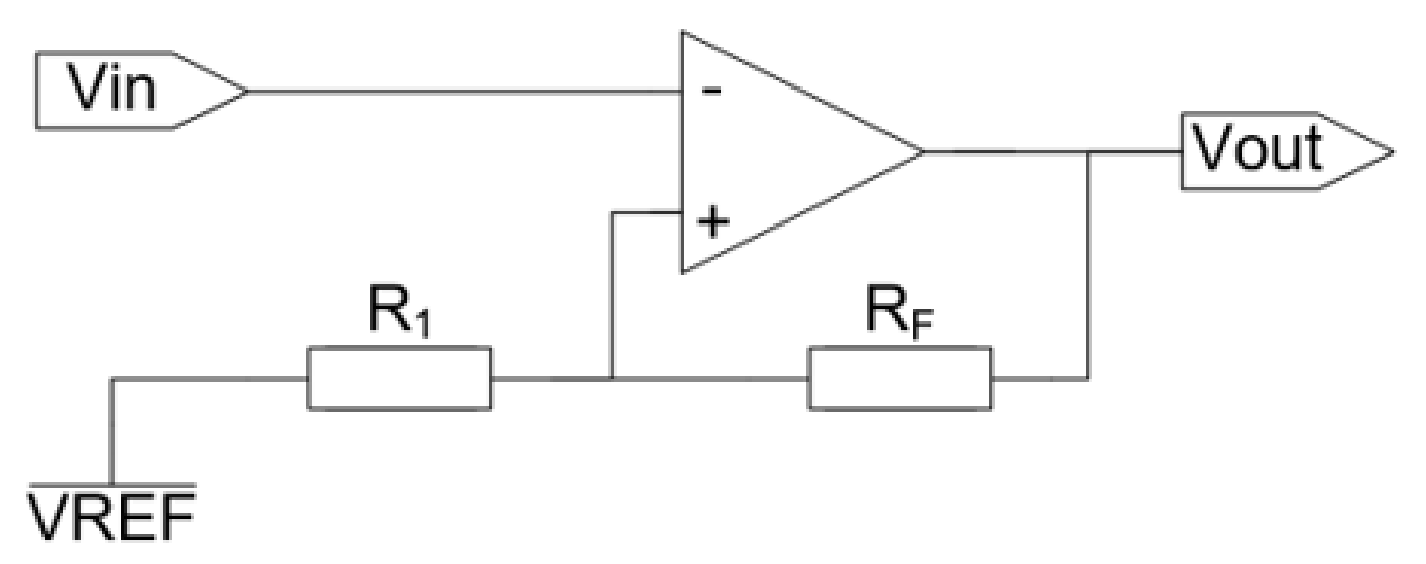
\includegraphics[width=4cm]{img/OpAmp/Schmitt-Trigger_invertierend.png}\\
  $V_{T_+} = V_{ref} + (V_{out max} - V_{ref})\frac{R_1}{R_1 + R_F} $ \\
  $V_{T_-} = V_{ref} + (V_{ref} - V_{out min})\frac{R_1}{R_1 + R_F} $\\
  $V_H = V_{T_+} - V_{T_-} = (V_{outmax} - V_{outmin})\frac{R_1}{R_1+R_F}$
\end{multicols}

\subsection{Nicht ideale OpAmps}
\begin{minipage}{0.49\textwidth}

  \small
  \subsubsection*{Offset-Spannung \& Begrenzte Verstärkung}
  \begin{itemize}[leftmargin=*]
    \item \textbf{Buffer}: \\
          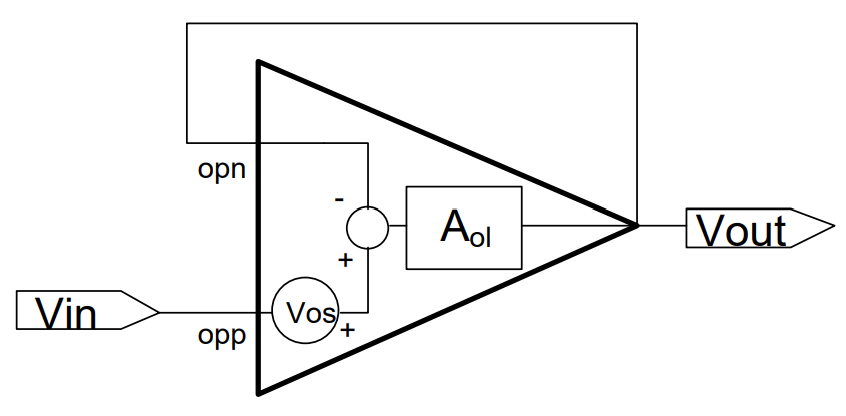
\includegraphics[width = 0.6 \textwidth]{img/OpAmp/NichtIdeal/Buffer.png}
          \\ $V_{out} = A_{ol} \cdot [(V_{in}+V_{os}) - V_{out}]$
          \\ $[A_{ol}\gg 1$ : $V_{out} = V_{in} + V_{os}]$
    \item \textbf{Verstärker}: \\
          \includegraphics[width = 0.6\textwidth]{img/OpAmp/NichtIdeal/verstärker.png}
          \\ $V_{out} = \frac{A_{ol}}{1+A_{ol}\cdot\frac{R_1}{R_1+R_2}}\cdot(V_{in}+V_{os}) $
          \\ $[A_{ol}\gg 1$: $V_{out} = \frac{R_1+R_2}{R_1}\cdot(V_{in}+V_{os})]$
    \item \textbf{Invertierender Verstärker}: \\
          \includegraphics[width = 0.6\textwidth]{img/OpAmp/NichtIdeal/invverstärker.png}
          \\ $V_{out} = \frac{A_{ol}}{1+A_{ol}\cdot\frac{R_1}{R_1+R_2}}\cdot[(V_{AGND} + V_{os})-V_{in}\cdot\frac{R_2}{R_1+R_2}]$
          \\ $[A_{ol}\gg 1$: $V_{out} = \frac{R_1 + R_2}{R_1}\cdot(V_{AGND}+V_{os})-\frac{R_2}{R_1}\cdot V_{in}]$
    \item \textbf{Allgemein}: \\
          $V_{out} = \frac{R1 + R2}{R1}\cdot(V_{agnd}+R_{os})-\frac{R2}{R1}\cdot V_{in}$
          \\ $V_{out-E-total} = A_{CL+} \cdot(|V_{os}| + \frac{|V_CM|}{CMRR} + \frac{|\Delta V_{Supply}|}{PSRR}) + |I_{OS}| \cdot R_F$
  \end{itemize}
\end{minipage}%
\begin{minipage}{0.49\textwidth}
  \begin{itemize}
    \item \textbf{Power Supply Rejection Ratio $PSRR$}
          \\ Unterdrückung der Beeinflussung durch \\ schwankende Speisespannung
          \\ $PSRR_{lin} = \frac{dV_{supply}}{dV_{os}}$
    \item \textbf{Common Mode Rejection Ratio $CMRR$}
          \\ Unterdrückung der Beeinflussung durch \\ schwankende Eingangsspannung
          \\ $V_{CM} = V_{opp} = V_{opn} \rightarrow CMRR_{lin} = \frac{dV_{CM}}{dV_{os}}$
  \end{itemize}
  \subsubsection*{Bias-Strom}
  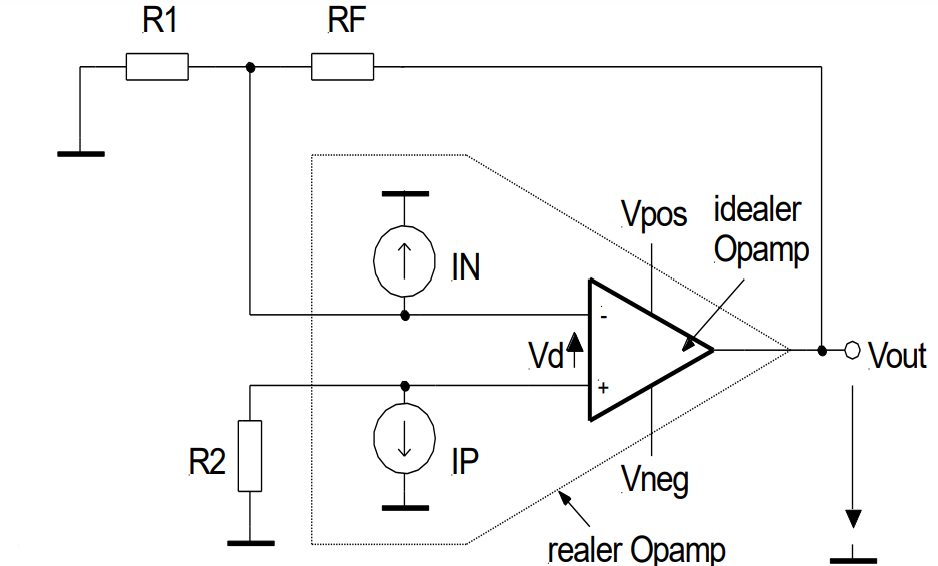
\includegraphics[height=3.5cm]{img/OpAmp/Fehler_Eingangsstrom.png}
  \\ \tiny{Rechnung mit Superposition:}\\
  $V_{out E} = I_NR_F-R_2I_P(\frac{R_F+R_1}{R_1}) $\\
  \textbf{Offset-Strom}
  $V_{out E} = R_F\cdot(I_N-I_P) = R_F\cdot I_{OS}$
  \subsubsection*{Einganswiderstände}
  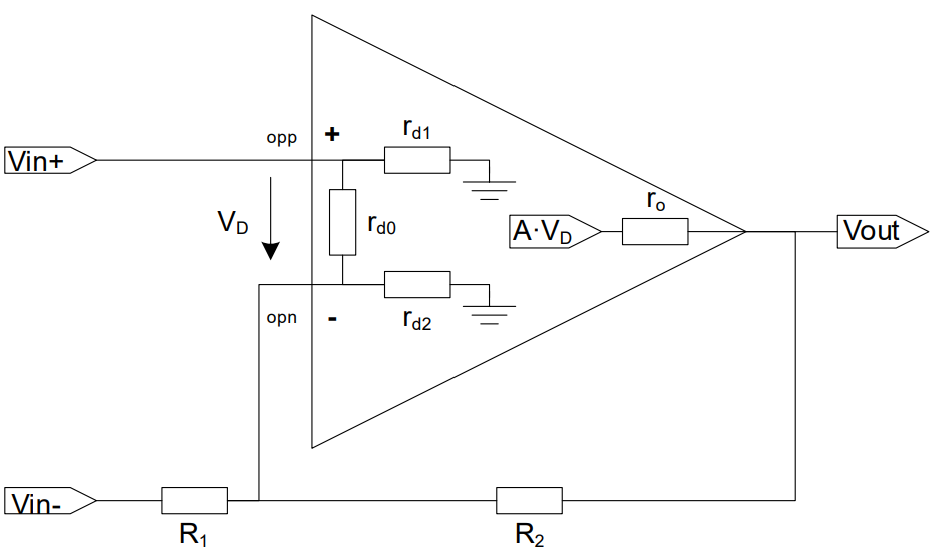
\includegraphics[height=3.5cm]{img/OpAmp/Fehler_Eingangswiderstand.png}\\
\end{minipage}


\section{Digital-/Analogwandler (DAC)}

\begingroup
\scriptsize
\subsubsection*{Wägeverfahren}
\begin{tabularx}{\textwidth}{p{0.25\textwidth}p{0.25\textwidth}
  p{0.25\textwidth}p{0.25\textwidth}}
  \textbf{Spannung}  &
  \textbf{Strom}     &
  \textbf{Kapazität} &
  \textbf{R-2R}
  \\ \includegraphics[width = 3cm]{img/DAC/Wägeverfahren.png}
                     &
  \raisebox{0.5\height}{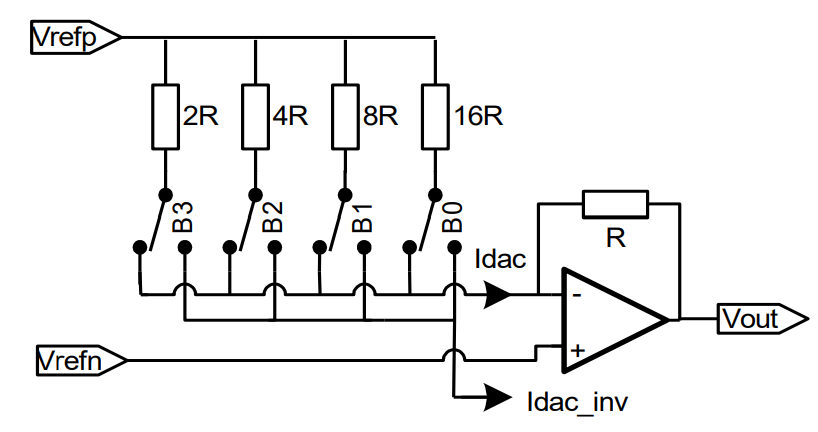
\includegraphics[width = 3cm]{img/DAC/Wägeverfahren_Ströme.png}}
                     &
  \raisebox{0.5\height}{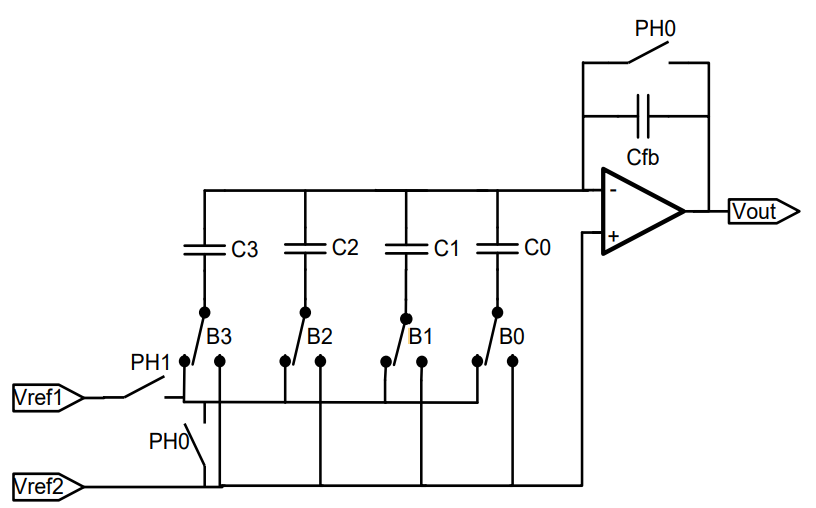
\includegraphics[width = 3cm]{img/DAC/C-DAC.png}}
                     &
  \raisebox{0.5\height}{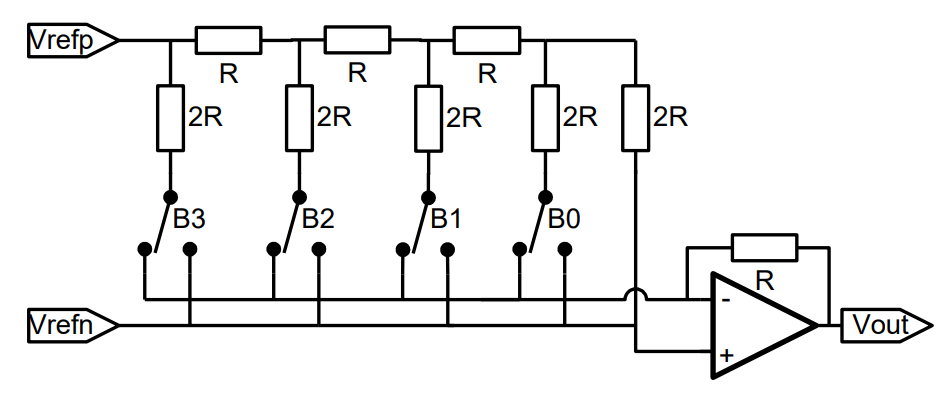
\includegraphics[width = 3cm]{img/DAC/R-2R-DAC.png}}
  \\
                     &
                     &
  \resizebox{0.25\textwidth}{!}{
    $V_{out} = (C_x) \cdot (V_{ref1} - V_{ref2} +) V_{ref2} $}
  \resizebox{0.25\textwidth}{!}{
    $Q_{CFB} = Q(C_x) = C_x \cdot (V_{ref1} - V_{ref2} + V_{ref2}) $}
  \resizebox{0.25\textwidth}{!}{
    $C_x = C_1 + C_2 \dots$
    (Alle aktiven Kapizitäten)}
                     &
  \scriptsize
  Jedes Bit leistet Beitrag:
  \newline 1. Bit $\frac{1}{2}$, 2. Bit $\frac{1}{4}$
  \newline n. Bit $\frac{1}{2^n} \Rightarrow V_{out} = \frac{X}{2^n}\cdot V_{ref}$
  \normalsize
\end{tabularx}
\endgroup
\subsection*{Weitere Verfahren}
\begingroup
\scriptsize
\begin{tabularx}{\textwidth}{p{0.33\textwidth}p{0.33\textwidth}p{0.33\textwidth}}
  \textbf{Parallelverfahren}
   &
  \textbf{Zählverfahren (PWM)}
   &
  \textbf{Kaskadiert}
  \\
  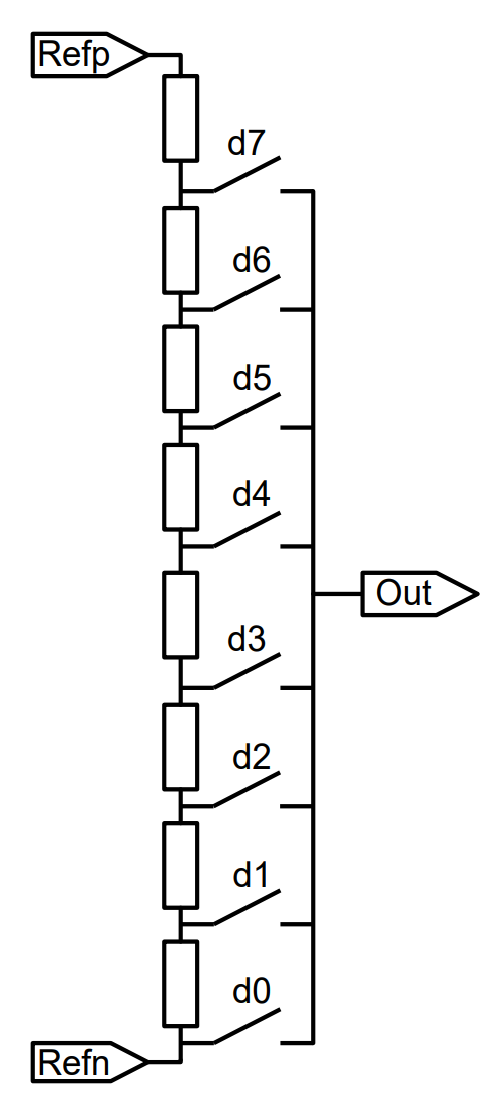
\includegraphics[height = 4cm,angle=90]{img/DAC/Parallelverfahren.png}
   &
  \includegraphics[width = 4cm]{img/DAC/DAC_mit_Zählverfahren.png}
  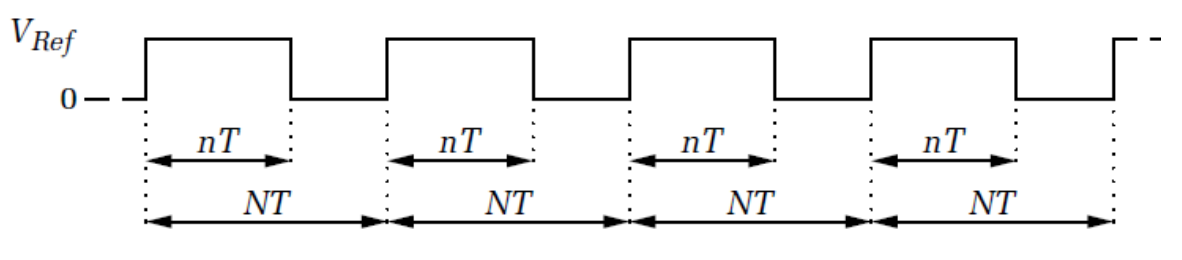
\includegraphics[width = 4cm]{img/DAC/PWM.png}
   &
  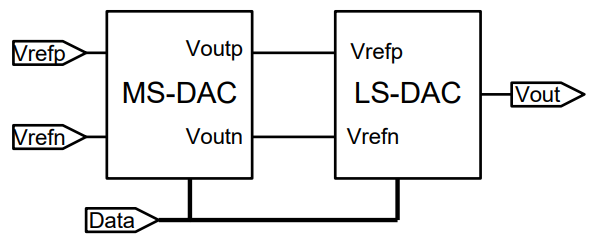
\includegraphics[width = 4cm]{img/DAC/Kaskadierte_Wandler.png}
  \\ %ParallelDac
  $V_{Ideal}(D) = \frac{D}{2^n} \cdot (V_{refp} - V_{refn} + V_{refn})$
  \newline
  \resizebox{0.33\textwidth}{!}{$V_{Real}(D) = \frac{\frac{D \cdot R_0 \cdot R_L}{D \cdot R_0 + R_L}}
      {(n-D) \cdot R_0 + \frac{D \cdot R_0 \cdot R_L}{D \cdot R_0 + R_L}} \cdot (V_{refp} - V_{refn}) $}
  \newline $q= \frac{1}{2^n} (V_{refp}-V_{refn})$
   &
  $\bar{V_{out} = V_{ref} \cdot \frac{n}{N}}$
  \newline
  {\tiny Geglättete Ausgangsspannung ergibt DC}
   &
  \\[20pt]
  \textbf{Zyklisch}
   &
  \textbf{Pipelined}
   &
  \textbf{Exponentiell}
  \\
  \raisebox{-\height}{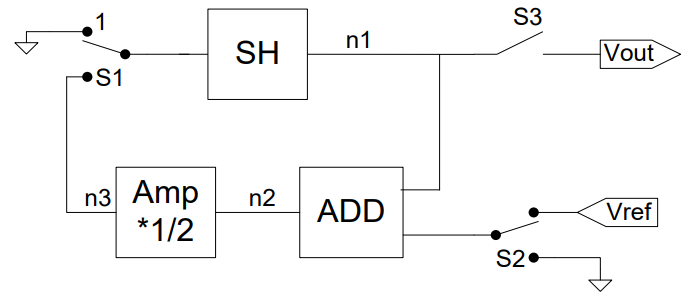
\includegraphics[width = 5cm]{img/DAC/Zyklischer_DAC.png}}
   &
  \raisebox{-\height}{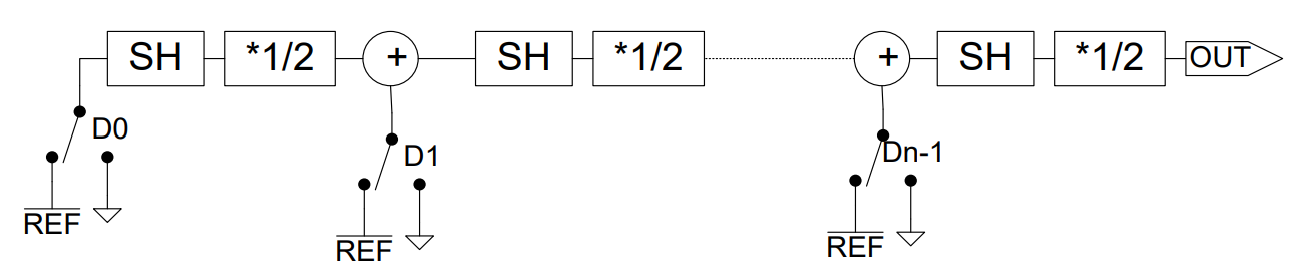
\includegraphics[width = 6cm]{img/DAC/Pipelined_DAC.png}}
   &
  \raisebox{-\height}{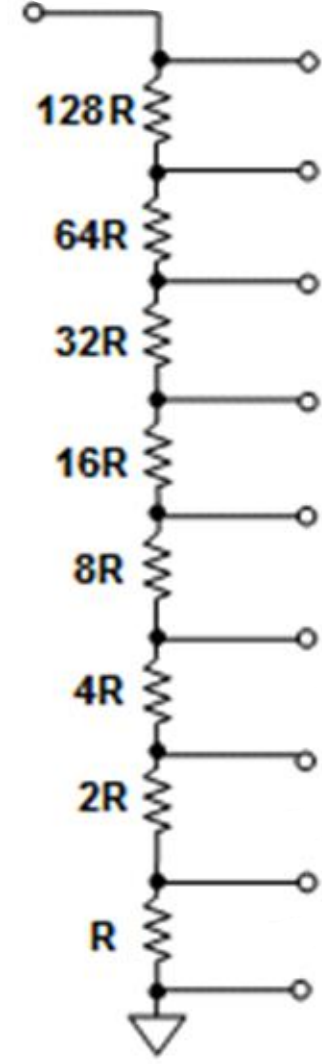
\includegraphics[height = 4cm,angle=90,origin=c]{img/DAC/Exponentieller_DAC.png}}
\end{tabularx}
\endgroup

\subsubsection*{Fehler}
\begingroup
\small
\begin{tabularx}{\textwidth}{p{0.2\textwidth}p{0.2\textwidth}p{0.2\textwidth}p{0.2\textwidth}p{0.2\textwidth}}
  \textbf{Offset}
   &
  \textbf{Verstärkungsfehler}
   &
  \textbf{Integrale \newline Nichtlinearität}
   &
  \textbf{Differentielle Nichtlinearität}
   &
  \textbf{Verzögerungszeit}
  \\
  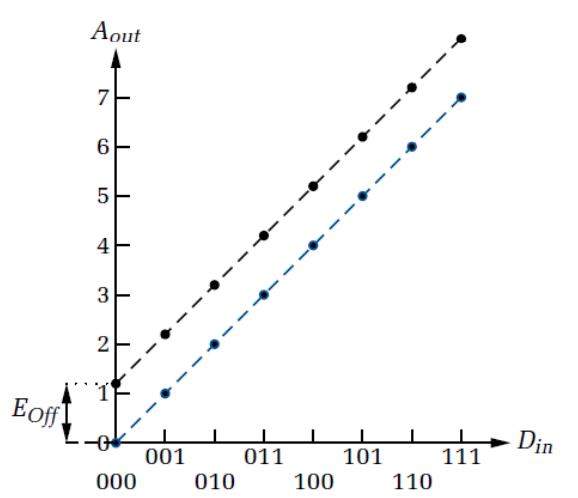
\includegraphics[width = 2cm]{img/DAC/Fehler/Offset.png}
   &
  \includegraphics[width = 2cm]{img/DAC/Fehler/Verstärkung.png}
   &
  \includegraphics[width = 2cm]{img/DAC/Fehler/IntegraleNichtlinearität.png}
   &
  \includegraphics[width = 2cm]{img/DAC/Fehler/DifferentielleNichtlinearität.png}
   &
  \includegraphics[width = 2cm]{img/DAC/Fehler/Verzögerungszeit.png}
\end{tabularx}
\endgroup

\section{Analog-Digital Wandler (ADC)}
\begin{tabular}{p{0.3\textwidth}p{0.3\textwidth}p{0.3\textwidth}}

  \textbf{Parallelverfahren}
  \newline 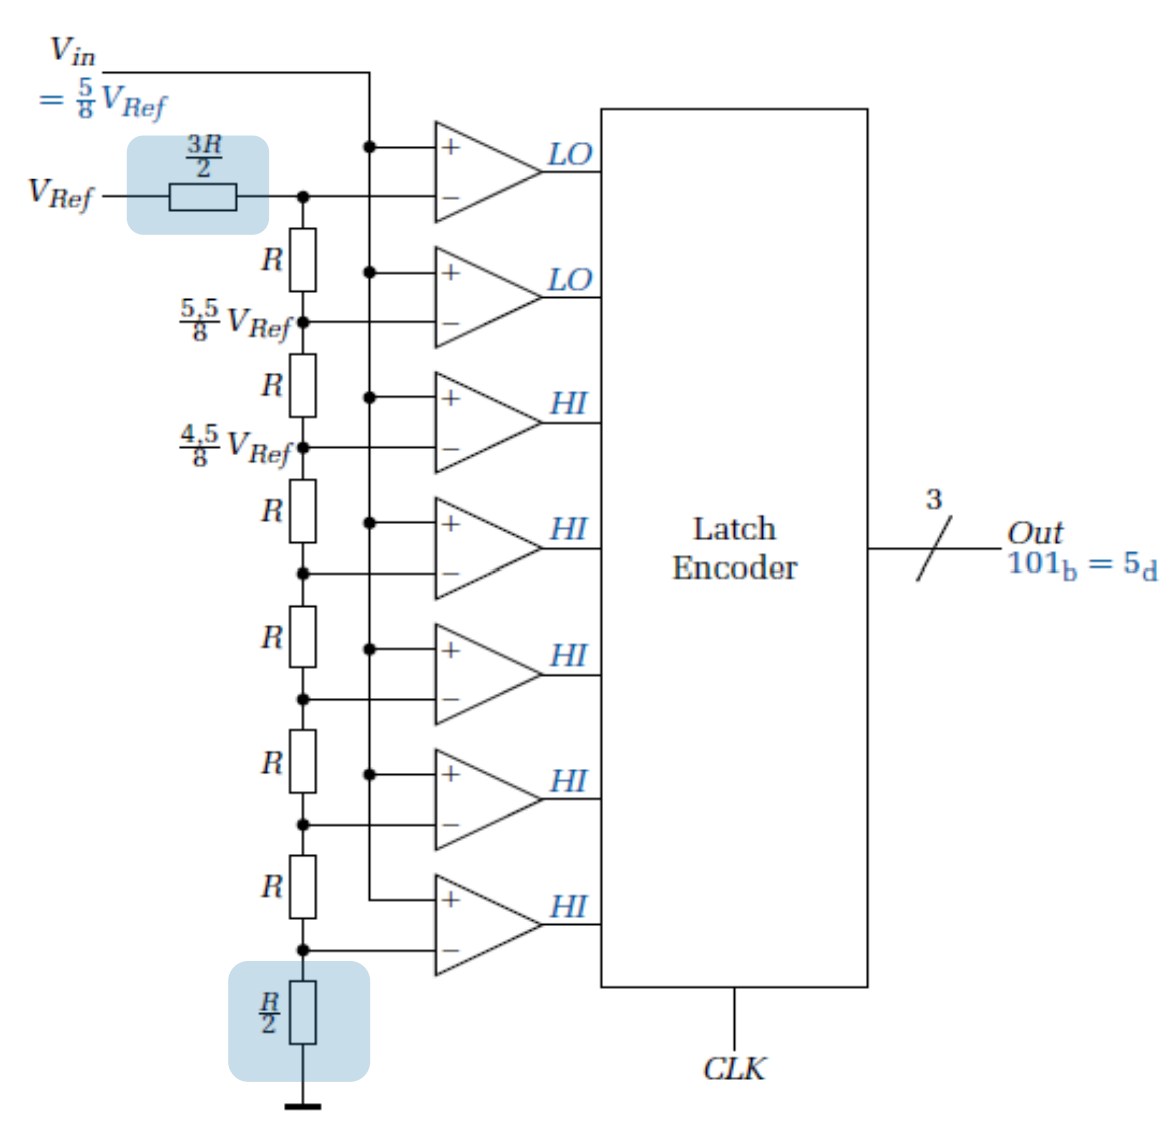
\includegraphics[width=0.2\textwidth,]{img/ADC/Parallel-Verfahren.png}
  \newline Pipeline-ADC
  \newline
  {\tiny Mit jeder Stufe wird ein Bit bestimmt}
  \newline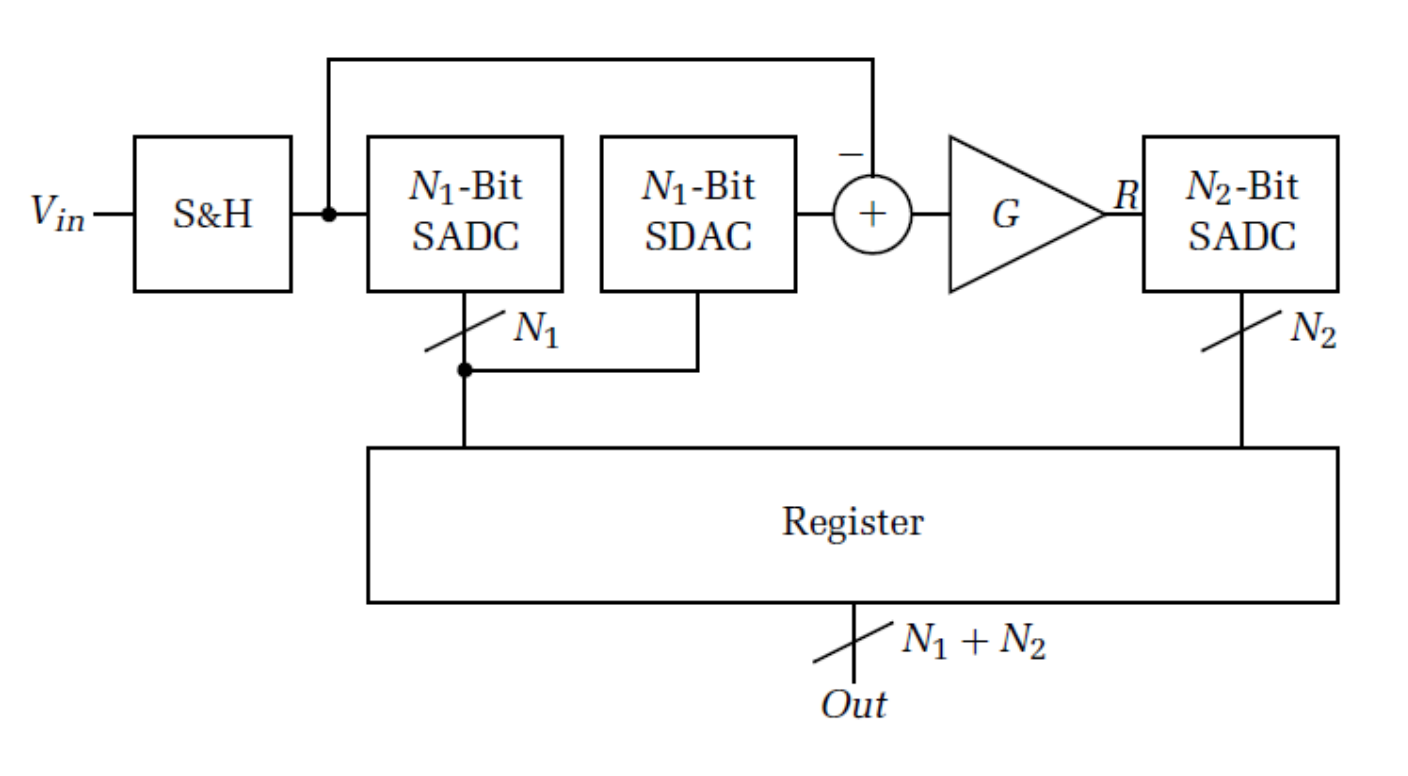
\includegraphics[width=0.3\textwidth]{img/ADC/Pipeline.png}

  Iterativer ADC
  \newline 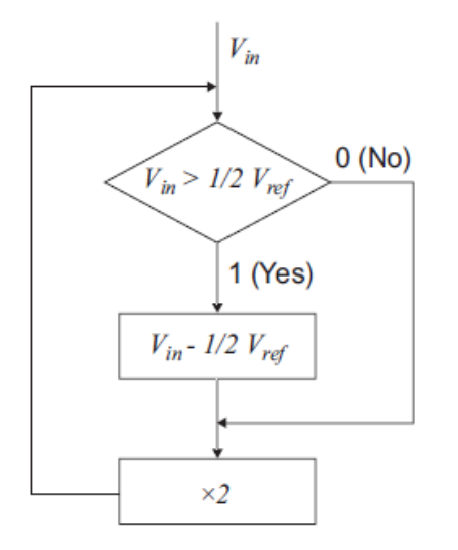
\includegraphics[width=0.3\textwidth]{img/ADC/IterativerADC.png}
   &
  \textbf{Wägeverfahren}
  \newline Succsessive Approximation Register (SAR)
  \newline\includegraphics[width=0.3\textwidth]{img/ADC/Wägeverfahren.png}
  {\tiny
  \newline 1. Sample Mode,
  \newline C werden auf $V_{in}$ geladen
  \newline 2. Holde Mode,
  \newline C werden auf Ground gelegt
  \newline $\Rightarrow V_x = -V_{in}$
  \newline 3. Redistribution Mode,
  \newline Schalter schliessen nacheinander
  \newline C bilden Spannungsteiler
  \newline $\Rightarrow V_x = -V_{in} + \frac{V_{ref}}{2} + \frac{V_{ref}}{4} \dots$
  \newline Wenn $V_x \leq 0\rightarrow \textrm{Bit} = 0$
  \newline Wenn $V_x > 0 \rightarrow \textrm{Bit} = 1$

  }
   &
  \textbf{Zählverfahren}
  \newline Single Slope Wandler
  \newline $V_{int}(t) = \frac{-V_{in}}{R\cdot C}\cdot t$
  \newline $V_{in} = \frac{V_{ref} \cdot R \cdot C}{T_{int}}$
  \newline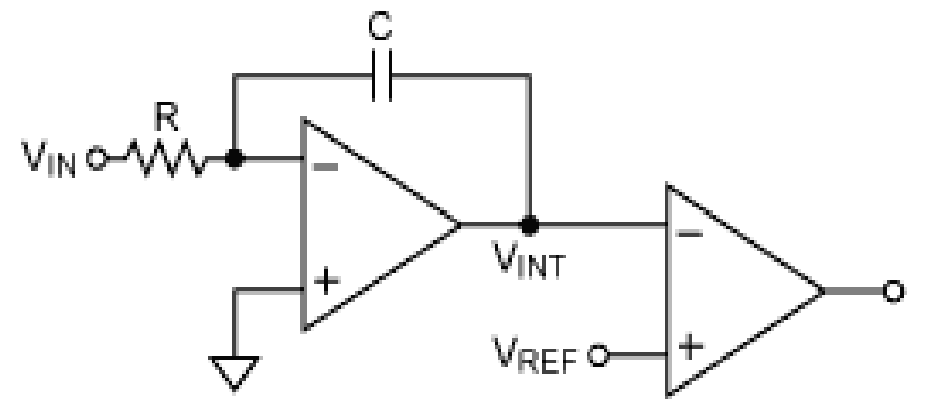
\includegraphics[width=0.3\textwidth]{img/ADC/SingleSlopeWandler.png}
  \newline Dual Slope Wandler
  \newline  $V_{int} = \int \limits ^{T_{int}} _0 -\frac{V_{in1}\cdot dt}{R_i \cdot C_i}$
  \newline $V_{int,max} = -\frac{\overline{V_{in}}\cdot T_{int}}{R_i \cdot C_i}$
  \newline $V_{int}(t) = V_{int,max}-\frac{V_{ref} \cdot t}{R_i \cdot C_i}$
  \newline $t_{abint} = -\frac{V_{in1}\cdot T_{int}}{V_{ref}}$

  \includegraphics[width=0.3\textwidth]{img/ADC/DualSlopeWandler.png}
\end{tabular}

\subsection{Fehler von ADC's}
\begin{tabularx}{\textwidth}{p{0.32\textwidth}p{0.32\textwidth}p{0.32\textwidth}}
  \textbf{Offset}
   &
  \textbf{Verstärkung-\newline Fehler}
   &
  \textbf{Integrale \newline Nichtlinearität}
  \\
  \includegraphics[width = 3.2cm]{img/ADC/OffsetFehler.png}
   &
  \includegraphics[width = 3.2cm]{img/ADC/Verstärkung.png}
   &
  \includegraphics[width = 3.2cm]{img/ADC/IntegraleNichtlinearität.png}
  \\
  \textbf{Differentielle Nichtlinearität}
   &
  \textbf{Quantisierung}
   &
  \textbf{Aliasing}
  \\
  \includegraphics[width = 3.2cm]{img/ADC/DifferentielleNichtlinearität.png}
   &
  \includegraphics[width = 3.2cm]{img/ADC/Quantisierungsfehler.png}
   &
  \includegraphics[width = 3.2cm]{img/ADC/Aliasing.png}
\end{tabularx}
\normalsize

\section{Halbleiter}
\subsection{Einführung}
\begin{multicols}{2}
  \subsubsection*{Elektrische Leitfähigkeit und Widerstand}
  $\kappa = \frac{1}{\rho} = n \cdot q \cdot \mu$
  \\$R = \rho \cdot \frac{l}{A} = \frac{l}{\kappa \cdot A} $
    {\\ \tiny \begin{itemize}[leftmargin=*]
          \item $\kappa$: Spezifische Leitfähigkeit
          \item $\rho$: Spezifischer Widerstand
          \item $n$: Ladungsträgerdichte
          \item $q$: Elementarladung
          \item $l$: Leiterlänge
          \item $A$: leiterquerschnittsfläche
        \end{itemize}}

    \subsubsection*{Temperaturabhängigkeit}
  $\rho = f(T)$
    \newline {\tiny annäherung 1. Ordnung:}
    \newline$\rho(T) = \rho(T_0) \cdot (1+ \alpha(T-T_0))$
  {\newline \tiny Tabelle im Anhang.}

  \subsubsection{Dotierung}
  {\tiny P-Dotiert: 3 Wertiges Element wird eingesetzt --> Löcher}
  \newline
  {\tiny N-Dotiert: 5 Wertiges Element wird eingesetzt --> Freie Elektronen}
\end{multicols}
\begin{multicols}{2}

  \subsection{Dioden}
  \includegraphics[width = 2cm]{img/Halbleiter/DifferenziellDiode.png}
  \includegraphics[width = 2cm]{img/Halbleiter/TemperaturkurvenDiode.png}
  {\tiny \begin{itemize}[leftmargin=*]
      \item $I_s$: Sättigungsstrom
      \item $n$: Emissionskoeffizient
      \item $I_D$: Diodenstrom ($A_{+} \rightarrow K_{-}$)
      \item $V_T$: Thermospannung bei Raumtemp. (25mV)
      \item $k$: Boltzmann Konstante
      \item $q$: Elementarladung
      \item $g$: Leitwert ($\frac{1}{R}$)
    \end{itemize}}

  \includegraphics[width = 3cm]{img/Halbleiter/Diode.png}
  \newline $V_T=\frac{kT}{q}$
  \newline $g = \frac{dl}{dV}
    = \frac{1}{n \cdot V_T} \cdot I_s \cdot e^{\frac{V}{n\cdot V_T}}
    = \frac{I}{n \cdot V_T}$
  \newline $I_d =I_s(e^{\frac{V_D}{nV_T}}-1)$
  \newline wenn $V_d > 200$mV: $I_d = I_s \cdot e^{\frac{V_d}{n \cdot V_t}}$
  \subsubsection*{DC-Ersatzschaltung (mit Vorwiderstand)}
  \includegraphics[width = 3cm]{img/Halbleiter/DCErsatzschaltungDiode.png}
  \small
  \newline$V_D = V_{D0} + (V_{src} - V_{D0} \cdot (\frac{R_D}{R_D + R1}))$
  \newline $R_D = \frac{\Delta U_D}{\Delta I_D}$
  \newline $V_{D0} =$ Schnittpunkt Linearisierung (Siehe Bild links)
  \normalsize
\end{multicols}

\newpage
\begin{minipage}{0.49\textwidth}
  \subsection{Bipolar-Transistor}
  $$I_E = I_C+I_B$$
  $$I_C = B\cdot I_B \approx \beta \cdot i_B$$
  $$I_B= I_s \cdot(e^{\frac{V_{BE}}{n \cdot V_T}}-1) \approx I_s e^{\frac{V_{BE}}{n \cdot V_T}}$$
  $$r_{BE} = \frac{\partial V_{BE}}{\partial I_B} \approx \frac{n \cdot V_T}{I_{B0}} $$

  {\tiny \begin{itemize}[leftmargin=*]
        \item C = Collector, E = Emitter, B = Basis
        \item $V_T$: Thermospannung bei Raumtemp. (25mV)
        \item $I_s$: Sättigungsstrom
        \item  $n$: Emissionskoeffizient
        \item $B$: Gleichstrom-Verstärkungsfaktor
        \item $\beta$: Wechselstrom-Verstärkungsfaktor
        \item Wird $V_{BE}$ um etwa 20mV erhöht verdoppelt sich $I_C$
      \end{itemize}}
\end{minipage}%
\begin{minipage}{0.49\textwidth}

  \subsubsection{Grundschaltungen einstufiger Verstärker}

  \begin{tabular}{p{3.51cm}p{3.51cm}}
    \textbf{Emitterschaltung}                                                                 &
    \textbf{Basisschaltung}                                                                     \\
    \raisebox{-\height}{\includegraphics[width = 3cm]{img/Transistor/Emitterschaltung.png}}   &
    \raisebox{-\height}{\includegraphics[width = 3cm]{img/Transistor/Basisschaltung.png}}       \\
    \textbf{Kollektorschaltung}                                                                 \\
    \raisebox{-\height}{\includegraphics[width = 3cm]{img/Transistor/Kollektorschaltung.png}} &
    Verstärkungen: \newline
    E: $\frac{I_C}{I_E} $ \newline
    B: $\frac{I_C}{I_B} $ \newline
    K: $\frac{I_E}{I_B} $
    \\
  \end{tabular}
\end{minipage}

\begin{minipage}{0.49\textwidth}

  \subsection{Emitterschaltung}
  \begin{itemize}[leftmargin=*]
    \item Für kleinere Toleranz: Emitterwiderstand einfügen
  \end{itemize}
  \includegraphics[width = 3.5cm]{img/Transistor/Verstärkung_Emitterschaltung.png}
  \includegraphics[width = 3.5cm]{img/Transistor/Uebertragungskennlinie.png}
  \subsubsection*{Grafische Herleitung Übertragungskennlinie}
  \begin{enumerate}
    \item $V_{BE} = V_{in}$
    \item Kein Ausgansstrom
          \\ $\rightarrow I_C = I_{RC} = \frac{V_{POS} - V_{out}}{R_C}$
    \item Kennlinie von $R_C$ einzeichnen
    \item Schnittpunkte sind mögliche Arbeitspunkte
  \end{enumerate}
  \subsubsection*{Berechnet}
  $$I_{RC} = \frac{V_{POS} - V_{out}}{R_C} = I_C = I_S \cdot \beta \cdot e^{\frac{V_{in}}{n \cdot V_T}}$$
  $$V_{out} = V_{POS}-R_C \cdot  I_S \cdot \beta \cdot e^{\frac{V_{in}}{n \cdot V_T}}$$
  {\\ \tiny git für $V_{CE-sat} < V_{out} < V_{POS}$}
  \subsubsection*{Verstärkung}
  $$V_{out} = V_{POS} - R_C \cdot \beta \cdot I_S \cdot e^{\frac{V_{in}}{n \cdot V_T}}$$
  Verstärkung = Ableitung $\frac{\Delta V_{out}}{\Delta V_{in}}$
  $$\frac{\partial V_{out}}{\partial V_{in}} =- R_C \cdot \beta \cdot I_S \cdot e^{\frac{V_{in}}{n \cdot V_T}} = \frac{-R_C \cdot I_C}{n \cdot V_T} $$
\end{minipage}%
\begin{minipage}{0.49\textwidth}
  \includegraphics[width = 0.5\textwidth]{img/Transistor/VerstärkerMitArbeitspunktanpassung.png}
  $$IB_0 = \frac{IC_0}{\beta}$$
  {\small ohne Bias-Strom (Strom durch R2)}
  $$V_{B0} = V_{POS} \frac{R_2}{R_1 + R_2}$$
  {\small mit Bias-Strom}
  $$V_B = \frac{R_2 \cdot V_{POS} - I_{B0} \cdot R_1 \cdot R_2}{R_1 + R_2}$$
  {\small Kleinsignal Verstärkung}
  $$A = -gm \cdot R_C = -\frac{I_{C0}}{n\cdot V_T}\cdot R_C$$
\end{minipage}
\begin{minipage}{0.49\textwidth}

  \subsection{Basisschaltung}
  \begin{itemize}[leftmargin=*]
    \item Bassisspannung Konstant
    \item Verwendung zur Stromsummierung
  \end{itemize}
  \includegraphics[width = 0.5\textwidth]{img/Transistor/Basisschaltung2.png}
  $$V_{out} = V_{POS} - R_C \cdot (\frac{V_E}{R_E} - \frac{\Delta V_{in}}{R_{in}}) = V_{out0} + \Delta V_{in} \frac{R_C}{R_{in}}$$
  $$\Delta I_{in} = \frac{\Delta V_{in}}{R_{in}} = \textrm{Wechselspannungssignal}$$
  $$\Delta V_{out} = \Delta I_{C} \cdot R_C = \Delta V_in \cdot \frac{R_C}{R_E}$$

\end{minipage}%
\begin{minipage}{0.5\textwidth}
  \subsection{Kollektorschaltung (Emitterfolger)}
  \begin{itemize}[leftmargin=*]
    \item Basis ist Eingang, Emitter is Ausgang
    \item Doppelter Strom wenn $\Delta B_{BE}$ ca. 20mV
    \item Spannungsverstärkung ~1
  \end{itemize}
  \includegraphics[width = 0.5\textwidth]{img/Transistor/Emitterschaltung2.png} %Bild falsch benannt!
  $$IC = \beta \cdot I_S \cdot e^{\frac{V_{BE}}{n \cdot V_T}}$$
  $$V_{out} = V_{in} - V_{BE} \approx V_{in} - 0.7V$$
\end{minipage}%

\subsection*{Modellierung von Transistoren}

\begin{minipage}{0.49\textwidth}
  \subsubsection*{VBE = VCE}
  \includegraphics[height = 50pt]{img/Transistor/VBEgleichVCETransistor.png}
  \includegraphics[height = 50pt]{img/Transistor/VBEgleichVCEErsatz.png}
  $R_{BE} = \frac{n \cdot V_T}{I_{B0}}$
  \subsubsection*{Ebers-Moll-Modell}
  \includegraphics[width = 0.8\textwidth]{img/Transistor/EbersMollModell.png}
\end{minipage}%
\begin{minipage}{0.49\textwidth}
  \subsubsection*{Kleinsignal-Modelle}
  \includegraphics[width = 0.8\textwidth]{img/Transistor/KleinsignalModell.png}
  $$r_{BE} = \frac{n \cdot V_T}{I_{B0}}$$
  $$\beta \cdot I_B = gm \cdot V_{BE} = \frac{\beta \cdot V_{BE}}{R_{BE}} = \frac{I_C\cdot V_{BE}}{n \cdot V_T}$$
  $$R_{CE} = \frac{V_A}{IC}$$
\end{minipage}%


\subsection*{Widlar Stromspiegel}
\includegraphics[width = 0.25\textwidth]{img/Transistor/Widlar.png}
\\$I_{out} = I_{in}$
\\bzw.
\\$I_{out} = I_{in} \cdot \frac{R_{E1}}{R_{E2}}$
\subsection{Leistungsverstärker / Ausgangsstufen}
\begin{minipage}{0.33\textwidth}
  \subsection*{Class A}
  \includegraphics[width = 0.5\textwidth]{img/Verstärker/ClassAVerstärker.png}
  $$\eta_{max} = \frac{P_{AC,max}}{P_{DC}} = 0.25\%$$
\end{minipage}%
\begin{minipage}{0.33\textwidth}
  \subsection*{Class B}
  \includegraphics[width = 0.5\textwidth]{img/Verstärker/ClassBVerstärker.png}
  $$\eta_{max} = \frac{P_{AC,max}}{P_{DC}} = \frac{\pi}{4} \approx 78.5\%$$
\end{minipage}%
\begin{minipage}{0.33\textwidth}
  \subsection*{Class AB}
  \includegraphics[width = 0.5\textwidth]{img/Verstärker/ClassABVerstärker.png}
  $$\eta \textrm{ kann nicht allgemein bestimmt werden.}$$
\end{minipage}%

\section*{Tabellen}
\textbf{Betriebszustände Transistor:}\\
\begin{tabular}{|c|c|c|c|}
  \hline
  $U_{BE}$ & $U_{BC}$ & Betriebszustände & Einsatzgebiete         \\
  \hline
  $>0$     & $<0$     & aktiv normal     & Verstärker             \\
  \hline
  $<0$     & $>0$     & aktiv invers     & -                      \\
  \hline
  $<0$     & $<0$     & gesperrt         & Schalter, Zustand: AUS \\
  \hline
  $>0$     & $>0$     & übersteuert      & Schalter, Zustand: EIN \\
  \hline
\end{tabular}
\\


\noindent \textbf{Eigenschaften typischer Stoffe:}\\
\begin{tabular}{|ccc|}
  \hline
  Material   & $\rho_{20}$ in $\frac{\Omega mm^2}{m}$ & $\alpha_{20}$ in $\frac{1}{K}$ \\[3pt]
  \hline
  Silber     & 0.016                                  & $3.8 \cdot 10^{-3}$            \\[3pt]
  \rowcolor[gray]{.9}
  Kupfer     & 0.0178                                 & $3.92 \cdot 10^{-3}$           \\[3pt]
  Gold       & 0.023                                  & $4 \cdot 10^{-3}$              \\[3pt]
  \rowcolor[gray]{.9}
  Aluminium  & 0.028                                  & $3.77 \cdot 10^{-3}$           \\[3pt]
  Konstantan & 0.43                                   & $\pm 40 \cdot 10^{-6}$         \\[3pt]
  \rowcolor[gray]{.9}
  Silizium   & $6.25 \cdot 10^6$                      & $-1\cdot 10^{-3} $             \\[3pt]
  Germanium  & $0.454 \cdot 10^6$                     & $-5\cdot 10^{-3} $             \\[3pt]
  \rowcolor[gray]{.9}
  Porzellan  & $5 \cdot 10^18$                        & -                              \\[3pt]
  \hline
\end{tabular}
\\

\noindent \textbf{Konstanten:} \\
\begin{tabular}{|lcl|}
  \hline
  Boltzmann Konstante & $k$        & $1.381 \cdot 10^{-23}$Ws/K \\[2pt]
  \rowcolor[gray]{.9}
  Elementarladung     & $q$        & $1.602 \cdot 10^{-19}$As   \\[2pt]
  Temparatur          & $^\circ C$ & $273.15$ K                 \\
  \hline
\end{tabular}



\end{document}














